\documentclass[12pt, twoside]{article}
\usepackage[utf8]{inputenc}
\usepackage[english,russian]{babel}

\usepackage{amsthm}
\usepackage{a4wide}
\usepackage{graphicx}
\usepackage{caption}
\usepackage{amssymb}
\usepackage{amsmath}
\usepackage{mathrsfs}
\usepackage{euscript}
\usepackage{graphicx}
\usepackage{subfig}
\usepackage{caption}
\usepackage{color}
\usepackage{bm}
\usepackage{tabularx}
\usepackage{adjustbox}


\usepackage[toc,page]{appendix}

\usepackage{comment}
\usepackage{rotating}

\DeclareMathOperator*{\argmax}{arg\,max}
\DeclareMathOperator*{\argmin}{arg\,min}

\newtheorem{theorem}{Теорема}
\newtheorem{lemma}[theorem]{Лемма}
\newtheorem{definition}{Определение}[section]

\numberwithin{equation}{section}

\newcommand*{\No}{No.}
\begin{document}

\title{\bf Анализ выбора априорного распределения для смеси экспертов \thanks{Работа выполнена при поддержке РФФИ и правительства РФ.}}
\date{}
\author{}
\maketitle

\begin{center}
\bf
А.\,В.~Грабовой\footnote{Московский физико-технический институт, grabovoy.av@phystech.edu}, В.\,В.~Стрижов\footnote{Московский физико-технический институт, strijov@ccas.ru}

\end{center}

{\centering\begin{quote}
\textbf{Аннотация:} 
Данная работа посвящен анализу свойств смеси экспертов в зависимости от выбора априорного распределения. Анализируется случай, когда выбрано информативное и неинформативное априорное распределения весов параметров каждого эксперта. В качестве экспертов рассматриваются линейные модели, а в качестве гипермодели рассматривается нейросеть с функцией softmax на последнем слое. В качестве базовой задачи рассматривается задача поиска окружностей на изображении. Предполагается, что каждой окружности на изображении соответсвует свой эксперт. В данной работе рассматривается случай, когда априорные распределения разных моделей являются независимы, а также случай, когда эти распределения являются зависимыми. В качестве данных рассматриваются синтетически сгенерированные окружности с разным уровнем шума. Сравнивается устойчивость к шуму мультимомделей с задаными априорными распределениями на вектора параметров локальных моделей и без задания априорного распределения.

\smallskip
\textbf{Ключевые слова}: смесь экспертов; байесовский выбор модели; априорное распределение.

\smallskip
\textbf{DOI}: 00.00000/00000000000000
\end{quote}
}

\section{Введение}
В данной работе рассматривается задача смеси экспертов. Смесь экспертов --- это мультимодель, которая линейно взвешивает локальных моделей аппроксимирующих выборку. Значение весовых коэффициенты зависят от того объекта для которого производится предсказание.

%Мультимодели показывают отличные результаты во многих задачах. 
Примерами мультимоделей являются беггинг и градиентный бустинг~\cite{Tianqi2016}, случайный лес~\cite{Ishwaran2012}. Подход к мультимоделированию~\cite{Yuksel2012} предполагает, что вклад каждой модели в ответ зависит от рассматриваемого объекта. Смесь экспертов использует шлюзовую функцию, которая определяет значимость предсказания каждого эксперта --- отдельной модели, входящей в смесь.

Для поиска оптимальных параметров мультимодели и локальных моделей рассматривается вероятностная постановка задачи. В качестве функционала качества рассматривается логарифм правдоподобия модели. Для оптимизации данного функционала рассматривается EM-алгоритм~\cite{Dempster1977}.

Мультимоделей имеют ряд недостатков, которые связаны с тем, что сходимость локальных моделей сильно зависит от начальной инициализации векторов параметров. Для улучшения сходимости предлагается использовать априорные знания. В данной работе задается априорное распределения на веса локальных моделей, также предлагается использовать зависимость априорных распределений, для улучшения качества мультимодели. 

\begin{figure}[h!t]\center
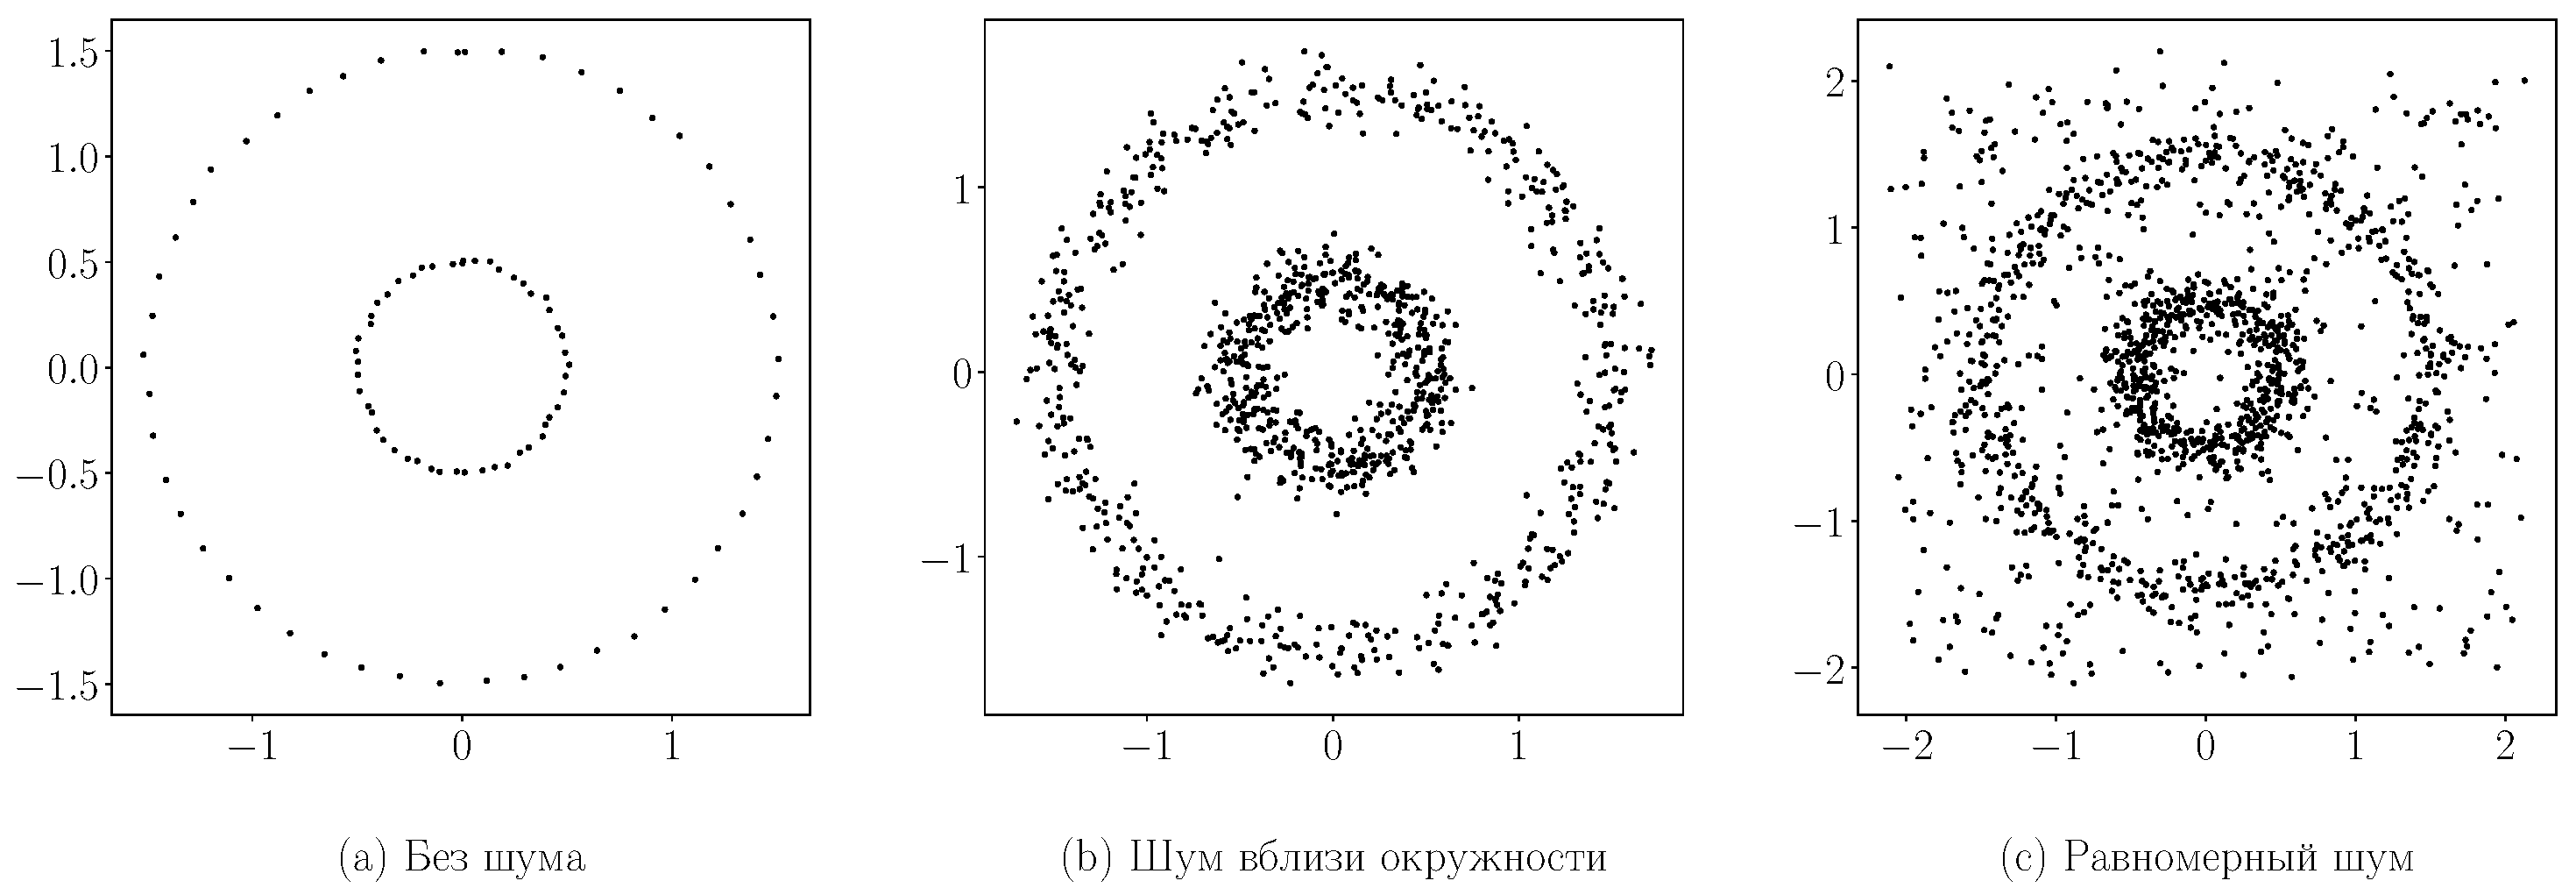
\includegraphics[width=1\textwidth]{result/statment}
\caption{Пример изображений с окружностями с разным уровнем шума: (a) окружности без шума; (b) окружности с зашумленным радиусом; (c) окружности с зашумленным радиусом, а также с равномерным шумом по всему изображению}
\label{example:1}
\end{figure}

Данная работа исследует зависимость качества модели в зависимости от выбора априорных распределений. Решается задача поиска окружностей на бинаризованном изображении. Предполагается, что радиусы окружностей различаются значимо, а также, что центры почти совпадают. Пример изображений показан на рис.~\ref{example:1}. Предлагается рассмотреть как ведет себя модель с априорными знанием и без них в случае изображений с разным уровнем шума. В данной работе в качестве отдельных экспертов рассматриваются линейные модели --- каждая модель отвечает своей окружности. В качестве шлюзовой функции рассматривается двухслойная нейронная сеть.

\section{Работы по теме}
Большое количество работ посвящены выбору шлюзовой функции: softmax--регрессия, процесс Дирихле~\cite{Edward2002}, нейронная сеть~\cite{Shazeer2017} с функцией softmax на последнем слое.

Ряд работ посвящены выбору моделей в качестве отдельных экспертов. В работах~\cite{Jordan1994, Jordan1991} в качестве модели эксперта рассматривается линейная модель. Работы~\cite{Lima2007, Cao2003} рассматриваю модель SVM в качестве модели эксперта.

В работа~\cite{Yuksel2012} представлен обзор методов и моделей в задачах смеси экспертов. В данной работе представлен обзор выше перечисленных шлюзовых функций. Также в данной работе проведен анализ разных моделей, которые могут выступать в качестве локальной модели.


\section{Постановка задачи нахождения параметров окружностей}
Задано бинарное изображение:
\begin{equation}
\label{eq:st:cr:1}
\begin{aligned}
\textbf{M} \in \{0,1\}^{m_1 \times m_2},
\end{aligned}
\end{equation}
где $0$ отвечает черной точке --- изображения, $1$ --- белой точке фона.

По изображению $\textbf{M}$ строится выборка $\textbf{C}$, элементами которой являются координаты~$x_i, y_i$ белых точек на картинке:
\begin{equation}
\label{eq:st:cr:2}
\begin{aligned}
\textbf{C} \in  \mathbb{R}^{N \times 2},
\end{aligned}
\end{equation}
где $N$ --- число черных точек на изображении $\textbf{M}$.

Обозначим $x_0, y_0$ --- центр окружности, которую требуется найти на бинарном изображении $\textbf{M}$, а $r$ ее радиус. Элементы выборки $\left(x_i, y_i\right)\in\textbf{C}$ являются геометрическим местом точек, которое заданное уравнение окружности окружности
\begin{equation}
\label{eq:st:cr:3}
\begin{aligned}
\left(x_i - x_0\right)^{2}+\left(y_i-y_0\right)^2 = r^2.
\end{aligned}
\end{equation}
Раскрыв скобки получим уравнение
\begin{equation}
\label{eq:st:cr:4}
\begin{aligned}
(2x_0)\cdot x_i + (2y_0)\cdot y_i+(r^2-x_0^2-y_0^2)\cdot1 = x_{i}^2 + y_{i}^2.
\end{aligned}
\end{equation}
Получаем задачу линейной регрессии для нахождения параметров окружности:
\begin{equation}
\label{eq:st:cr:5}
\begin{aligned}
\textbf{X}\textbf{w} \approx \textbf{y},  \quad \textbf{X} = \textbf{C}\times \textbf{1}, \quad \textbf{y} = [x_1^2+y_1^2, x_2^2+y_2^2, \cdots, x_N^2+y_N^2]^{\mathsf{T}},
\end{aligned}
\end{equation}
где найденые оптимальные параметры линейной регрессии $\textbf{w} = \bigr[w_1, w_2, w_3\bigr]^{\mathsf{T}}$ восстанавливают параметры окружности:
\begin{equation}
\label{eq:st:cr:6}
\begin{aligned}
x_0 = \frac{w_1}{2}, \quad y_0 = \frac{w_2}{2}, \quad r = \sqrt[]{w_3+x_{0}^{2}+y_{0}^{2}}.
\end{aligned}
\end{equation}

Решение уравнения~\eqref{eq:st:cr:5} находит параметры единственной окружности на изображении. В случае, когда на изображении несколько окружностей, предлагается использовать мультимодель. В ее состав входят линейные модели Каждая линейная модель описывает одну окружность на изображении. В качестве мультимодели рассматривается смесь экспертов.

\section{Постановка задачи построения смеси экспертов}

Задана выборка из~\eqref{eq:st:cr:5} 
\begin{equation}
\label{eq:st:1}
\begin{aligned}
\textbf{X} \in \mathbb{R}^{N \times n},
\end{aligned}
\end{equation}
где~$N$~---~число объектов в выборке, а~$n$~---~размерность признакового пространства.

\begin{definition}
\label{def:1}
Смесь экспертов~---~мультимодель, определяющая правдоподобие веса $\pi_k$ каждой локальной модели $\textbf{f}_k$ на признаковом описании объекта $\textbf{x}$.

\begin{equation}
\label{eq:st:2}
\begin{aligned}
\hat{\mathbf{f}} = \sum_{k=1}^{K}\pi_{k}\mathbf{f}_k, \qquad \pi_{k}\left(\mathbf{x}, \mathbf{V}\right):\mathbb{R}^{n\times \left|\mathbf{V}\right|} \to [0, 1], \qquad \sum_{k=1}^{K}\pi_{k}\left(\mathbf{x}, \mathbf{V}\right) = 1
\end{aligned}
\end{equation}
где~$\hat{\mathbf{f}}$~---~мультимодель, а $\mathbf{f}_k$ является некоторой моделью, $\pi_k$~---~параметрическая модель, $\mathbf{w}_k$~---~параметры $k$-й локальной модели, $\mathbf{V}$~---~параметры шлюзовой функции.
\end{definition}

В данной работе в качестве локальных моделей~$\mathbf{f}_k$ и шлюзовой функции~$\bm{\pi}$ рассматриваются следующие функции:
\begin{equation}
\label{eq:st:3}
\begin{aligned}
\mathbf{f}_k\left(\textbf{x}\right) = \textbf{w}_k^{\mathsf{T}}\textbf{x}, \quad
\bm{\pi}\left(\mathbf{x}, \mathbf{V}\right) = \text{softmax}\bigr(\mathbf{V}_{1}^{\mathsf{T}}\bm{\sigma}\left(\mathbf{V}_2^{\mathsf{T}}\mathbf{x}\right)\bigr),
\end{aligned}
\end{equation}
где $\mathbf{V} = \bigr[\mathbf{V}_1, \mathbf{V}_2\bigr]$~---~параметры шлюзовой функции.

В качестве функционала качества рассматривается правдоподобие модели:
\begin{equation}
\label{eq:st:4}
\begin{aligned}
p\bigr(\mathbf{y}, \mathbf{W}|\mathbf{X}, \mathbf{V}\bigr) = \prod_{k=1}^{K}p^{k}\bigr(\mathbf{w}_k\bigr)\prod_{i=1}^{N}\left(\sum_{k=1}^{K}\pi_{k}p_{k}\bigr(y_i|\mathbf{w}_k, \mathbf{x}_i\bigr)\right),
\end{aligned}
\end{equation}
где $\mathbf{W} = \bigr[\mathbf{w}_1, \mathbf{w}_2, \cdots, \mathbf{w}_K\bigr]^{\mathsf{T}}$

Получаем следующую задачу оптимизации:
\begin{equation}
\label{eq:st:5}
\begin{aligned}
\mathbf{W}, \mathbf{V} = \arg\max_{\mathbf{W}, \mathbf{V}} p\bigr(\mathbf{y}, \mathbf{W}|\mathbf{X}, \mathbf{V}\bigr)
\end{aligned}
\end{equation}

\section{EM--алгоритм для решения задачи смеси экспертов}
Рассмотрим следующую вероятностную постановку задачи:
\begin{enumerate}
	\item $p_{k}\left(y_{i}|\mathbf{w}_{k}, \mathbf{x}_{i}\right) = \mathcal{N}\left(y_{i}|\mathbf{w}_{k}^{\mathsf{T}}\mathbf{x}_{i}, \beta^{-1}\right)$
	\item $p^{k}\left(\mathbf{w}_{k}\right) = \mathcal{N}\left(\mathbf{w}_{k}|\mathbf{w}^{0}_{k}, \mathbf{A}_{k}\right)$
	\item $p\left(\bm{\varepsilon}_{k,k'}|\bm{\alpha}\right) = \mathcal{N}\left(\bm{\varepsilon}_{k,k'}|\mathbf{0},  \hat{\bm{\alpha}}\right),$ где $\bm{\varepsilon}_{k,k'} = \mathbf{w}_{k}^{0}-\mathbf{w}_{k'}^{0},$ $\hat{\bm{\alpha}} = \text{diag}\left(\bm{\alpha}\right)$~---~диагональная матрица, диагональ которой равняется~$\bm{\alpha}$.
\end{enumerate}
Тогда правдоподобия модели~\eqref{eq:st:4} переписывается в следующем виде:
\begin{equation}
\label{eq:em:1}
\begin{aligned}
p\bigr(\mathbf{y}, \mathbf{W}|\mathbf{X}, \mathbf{V}, \textbf{A}, \textbf{W}^{0}, \hat{\bm{\alpha}}, \beta\bigr) = &\prod_{k,k'=1}^{K}\mathcal{N}\left(\bm{\varepsilon}_{k,k'}|\mathbf{0},  \hat{\bm{\alpha}}\right)\cdot\\
&\cdot\prod_{k=1}^{K}\mathcal{N}\left(\mathbf{w}_{k}|\mathbf{w}^{0}_{k}, \mathbf{A}_{k}\right)\prod_{i=1}^{N}\left(\sum_{k=1}^{K}\pi_{k}\mathcal{N}\left(y_{i}|\mathbf{w}_{k}^{\mathsf{T}}\mathbf{x}_{i}, \beta^{-1}\right)\right),
\end{aligned}
\end{equation}
где~$\mathbf{A} = \bigr[\mathbf{A}_1, \cdots, \mathbf{A}_K\bigr]$

Для решения задачи~\eqref{eq:st:5} в условиях правдоподобия~\eqref{eq:em:1} введем матрицу скрытых переменных~$\mathbf{Z}$, где $z_{ik} = 1$, если $i$-й~объект порожден моделью~$k$ и~$z_{ik} = 0$ иначе. Используя~$\mathbf{Z}$, логарифм правдоподобие~\eqref{eq:em:1} переписывается следующим образом:

\begin{equation}
\label{eq:em:2}
\begin{aligned}
\log p\bigr(\mathbf{y}, \mathbf{Z}, \mathbf{W}&|\mathbf{X}, \mathbf{V}, \textbf{A}, \textbf{W}^{0}, \hat{\bm{\alpha}}, \beta\bigr) =\\
&= \sum_{i=1}^{N}\sum_{k=1}^{K}z_{ik}\left[\log\pi_k\left(\textbf{x}_i, \textbf{V}\right) - \frac{\beta}{2}\left(y_{i} - \textbf{w}_{k}^{\mathsf{T}}\textbf{x}_{i}\right)^{2} + \frac{1}{2}\log\frac{\beta}{2\pi}\right] +\\
&+ \sum_{k=1}^{K}\left[-\frac{1}{2}\left(\textbf{w}_{k} - \textbf{w}_{k}^{0}\right)^{\mathsf{T}}\textbf{A}_{k}^{-1}\left(\textbf{w}_{k} - \textbf{w}_{k}^{0}\right) + \frac{1}{2}\log\det\textbf{A}^{-1}_{k} - \frac{n}{2}\log2\pi\right]+\\
&+ \sum_{k=1}^{K}\sum_{k'=1}^{K}\left[-\frac{1}{2}\left(\textbf{w}_{k}^{0}-\textbf{w}_{k'}^{0}\right)^{\mathsf{T}}\hat{\bm{\alpha}}^{-1}\left(\textbf{w}_{k}^{0}-\textbf{w}_{k'}^{0}\right) +\frac{1}{2}\log\det\hat{\bm{\alpha}} -\frac{n}{2}\log{2\pi}\right].
\end{aligned}
\end{equation}
С учетом~\eqref{eq:em:2} задача оптимизации~\eqref{eq:st:5} принимает вид:
\begin{equation}
\label{eq:em:3}
\begin{aligned}
\mathbf{W}, \mathbf{Z}, \mathbf{V}, \mathbf{W}^0, \textbf{A},  \beta = \arg\max_{\mathbf{W}, \mathbf{Z}, \mathbf{V}, \mathbf{W}^0, \textbf{A}, \beta} \log p\bigr(\mathbf{y}, \mathbf{Z}, \mathbf{W}&|\mathbf{X}, \mathbf{V}, \textbf{A}, \textbf{W}^{0}, \hat{\bm{\alpha}}, \beta\bigr)
\end{aligned}
\end{equation}

Для поиска локального минимума в задаче оптимизации~\eqref{eq:em:3} воспользуемся EM-алгоритмом.

\paragraph{E--step.} Найдем $q\left(\mathbf{Z}, \mathbf{W}\right) = q\left(\mathbf{Z}\right)q\left(\mathbf{W}\right)$ найболее близкое к $p\bigr(\mathbf{Z}, \mathbf{W}|\mathbf{y}, \mathbf{X}, \mathbf{V}, \textbf{A}, \textbf{W}^{0}, \hat{\bm{\alpha}}, \beta\bigr)$.

\begin{equation}
\label{eq:em:4}
\begin{aligned}
\log q\left(\textbf{Z}\right) &= \mathsf{E}_{q/\textbf{Z}} \log p\bigr(\mathbf{y}, \mathbf{Z}, \mathbf{W}|\mathbf{X}, \mathbf{V}, \textbf{A}, \textbf{W}^{0}, \hat{\bm{\alpha}}, \beta\bigr)  \propto\\
&\propto \sum_{i+1}^{N}\sum_{k=1}^{K}z_{ik}\left[\log\pi_{k}\left(\textbf{x}_{i}, \textbf{V}\right) - \frac{\beta}{2}\left(y_{i}^{2} -\textbf{x}_{i}^{\mathsf{T}}\mathsf{E}\textbf{w}_{k} + \textbf{x}_{i}^{\mathsf{T}}\mathsf{E}\textbf{w}_{k}\textbf{w}_{k}^{\mathsf{T}}\textbf{x}_{i}\right) + \frac{1}{2}\log\frac{\beta}{2\pi}\right]\\
p\left(z_{ik} = 1\right) &= \frac{\exp\left(\log\pi_{k}\left(\textbf{x}_{i}, \textbf{V}\right) - \frac{\beta}{2}\left(\textbf{x}_{i}^{\mathsf{T}}\mathsf{E}\textbf{w}_{k}\textbf{w}_{k}^{\mathsf{T}}\textbf{x}_{i} - \textbf{x}_{i}^{\mathsf{T}}\mathsf{T}\textbf{w}_{k}\right)\right)}{\sum_{k'=1}^{K}\exp\left(\log\pi_{k'}\left(\textbf{x}_{i}, \textbf{V}\right) - \frac{\beta}{2}\left(\textbf{x}_{i}^{\mathsf{T}}\mathsf{E}\textbf{w}_{k'}\textbf{w}_{k'}^{\mathsf{T}}\textbf{x}_{i} - \textbf{x}_{i}^{\mathsf{T}}\mathsf{T}\textbf{w}_{k'}\right) \right)}
\end{aligned}
\end{equation}

Получаем, что параметр $q\bigr(z_{ik}\bigr)$ является Бернулевской случайной величиной с параметров заданным в выражении~\eqref{eq:em:4}.

\begin{equation}
\label{eq:em:5}
\begin{aligned}
\log q\left(\textbf{W}\right) &= \mathsf{E}_{q/\textbf{W}}\log p\bigr(\mathbf{y}, \mathbf{Z}, \mathbf{W}|\mathbf{X}, \mathbf{V}, \textbf{A}, \textbf{W}^{0}, \hat{\bm{\alpha}}, \beta\bigr) \propto\\
&\propto \sum_{i=1}^{N}\sum_{k=1}^{K}\mathsf{E}z_{ik}\left[\log\pi_{k}\left(\textbf{x}_{i, \textbf{V}}\right) - \frac{\beta}{2}\left(y_{i} - \textbf{w}_{k}^{\mathsf{T}}\textbf{x}_{i}\right)^{2} + \frac{1}{2}\log\frac{\beta}{2\pi}\right] + \\
&+ \sum_{k=1}^{K}\left[-\frac{1}{2}\left(\textbf{w}_{k} - \textbf{w}_{k}^{0}\right)^{\mathsf{T}}\textbf{A}_{k}^{-1}\left(\textbf{w}_{k} - \textbf{w}_{k}^{0}\right) + \frac{1}{2}\log\det\textbf{A}^{-1}_{k} - \frac{n}{2}\log2\pi\right] \\
&\propto \sum_{k=1}^{K}\left[\textbf{w}_{k}^{\mathsf{T}}\left(\textbf{A}_{k}^{-1}\textbf{w}_{k}^{0}+\beta\sum_{i=1}^{N}\textbf{x}_{i}y_{i}\mathsf{E}z_{ik}\right)-\frac{1}{2}\textbf{w}_{k}^{\mathsf{T}}\left(\textbf{A}_{k}^{-1}+\beta\sum_{i=1}^{N}\textbf{x}_{i}\textbf{x}_{i}^{\mathsf{T}}\right)\textbf{w}_{k}\right]
\end{aligned}
\end{equation}

Получаем, что распределение $q\bigr(\mathbf{w}_{k}\bigr) = \mathcal{N}\left(\mathbf{w}_{k}| \mathbf{m}_{k}, \mathbf{B}_k\right),$ где параметры $\mathbf{m}_k, \mathbf{B}_k$ определяются следующим образом:
\begin{equation}
\label{eq:em:6}
\begin{aligned}
\mathbf{m}_{k} = \mathbf{B}_{k}\left(\mathbf{A}_{k}^{-1}\mathbf{w}_{k}^{0}+\beta\sum_{i=1}^{N}\mathbf{x}_{i}y_{i}\mathsf{E}z_{ik}\right) \qquad \mathbf{B}_{k} = \left(\mathbf{A}_{k}^{-1}+\beta\sum_{i=1}^{N}\mathbf{x}_{i}\mathbf{x}_{i}^{\mathsf{T}}\mathsf{E}z_{ik}\right)^{-1} 
\end{aligned}
\end{equation}

\paragraph{M--step.} Найдем $\mathbf{V}, \mathbf{W}^0, \textbf{A},  \beta$ из максимизации~$\mathsf{E}_{q}\log p\bigr(\mathbf{y}, \mathbf{Z}, \mathbf{W}|\mathbf{X}, \mathbf{V}, \textbf{A}, \textbf{W}^{0}, \hat{\bm{\alpha}}, \beta\bigr)$.

\begin{equation}
\label{eq:em:7}
\begin{aligned}
\mathcal{F}\left(\textbf{V}, \textbf{W}^{0}, \textbf{A}, \beta\right) &= \mathsf{E}_{q}\log p\bigr(\mathbf{y}, \mathbf{Z}, \mathbf{W}|\mathbf{X}, \mathbf{V}, \textbf{A}, \textbf{W}^{0}, \hat{\bm{\alpha}}, \beta\bigr) =  \\
&= \sum_{i=1}^{N}\sum_{k=1}^{K}\mathsf{E}z_{ik}\left[\log\pi_k\left(\textbf{x}_i, \textbf{V}\right) - \frac{\beta}{2}\mathsf{E}\left(y_{i} - \textbf{w}_{k}^{\mathsf{T}}\textbf{x}_{i}\right)^{2} + \frac{1}{2}\log\frac{\beta}{2\pi}\right] +\\
&+ \sum_{k=1}^{K}\left[-\frac{1}{2}\mathsf{E}\left(\textbf{w}_{k} - \textbf{w}_{k}^{0}\right)^{\mathsf{T}}\textbf{A}_{k}^{-1}\left(\textbf{w}_{k} - \textbf{w}_{k}^{0}\right) + \frac{1}{2}\log\det\textbf{A}^{-1}_{k} - \frac{n}{2}\log2\pi\right] +\\
&+ \sum_{k=1}^{K}\sum_{k'=1}^{K}\left[-\frac{1}{2}\left(\textbf{w}_{k}^{0}-\textbf{w}_{k'}^{0}\right)^{\mathsf{T}}\hat{\bm{\alpha}}^{-1}\left(\textbf{w}_{k}^{0}-\textbf{w}_{k'}^{0}\right) +\frac{1}{2}\log\det\hat{\bm{\alpha}} -\frac{n}{2}\log{2\pi}\right].
\end{aligned}
\end{equation}

Так-как~$\mathcal{F}\left(\textbf{V}, \textbf{W}^{0}, \textbf{A}, \beta\right)$ является вогнутой, то для нахождения оптимальных параметров воспользуемся условием первого порядка.

\begin{equation}
\label{eq:em:8}
\begin{aligned}
	\frac{\partial \mathcal{F}\left(\textbf{V}, \textbf{W}^{0}, \textbf{A}, \beta\right)}{\partial \textbf{V}} = 0
\end{aligned}
\end{equation}

Решение уравнения~\eqref{eq:em:8} найдем при помощи градиентного метода оптимизации, которое гарантирует сходимость к локальному экстремуму функции~$\mathcal{F}\left(\textbf{V}, \textbf{W}^{0}, \textbf{A}, \beta\right)$.

\begin{equation}
\label{eq:em:9}
\begin{aligned}
\frac{\partial \mathcal{F}\left(\textbf{V}, \textbf{W}^{0}, \textbf{A}, \beta\right)}{\partial \textbf{A}^{-1}_k} &=  \frac{1}{2}\textbf{A}_{k} - \frac{1}{2}\mathsf{E}\left(\textbf{w}_{k} - \textbf{w}_{k}^{0}\right)\left(\textbf{w}_{k} - \textbf{w}_{k}^{0}\right)^{T} = 0\\
\textbf{A}_{k} &= \mathsf{E}\textbf{w}_{k}\textbf{w}_{k}^{\mathsf{T}} - \textbf{w}_{k}^{0}\mathsf{E}\textbf{w}_{k}^{\mathsf{T}} - \mathsf{E}\textbf{w}_{k}\textbf{w}_{k}^{0\mathsf{T}} + \textbf{w}_{k}^{0}\textbf{w}_{k}^{0\mathsf{T}} 
\end{aligned}
\end{equation}


\begin{equation}
\label{eq:em:10}
\begin{aligned}
\frac{\partial \mathcal{F}\left(\textbf{V}, \textbf{W}^{0}, \textbf{A}, \beta\right)}{\partial \beta} &= \sum_{k=1}^{K}\sum_{i=1}^{N}\left(\frac{1}{\beta}\mathsf{E}z_{ik}-\frac{1}{2}\mathsf{E}z_{ik}\left[y_{i}^{2}-2y_{i}\textbf{x}_{i}^{\mathsf{T}}\mathsf{E}\textbf{w}_{k}+\textbf{x}_{i}^{\mathsf{T}}\textbf{w}_{k}\textbf{w}_{k}^{\mathsf{T}}\textbf{x}_{i}\right]\right) = 0\\
\frac{1}{\beta}&=\frac{1}{N}\sum_{i=1}^{N}\sum_{k=1}^{K}\left[y_{i}^{2}-2y_{i}\textbf{x}_{i}^{\mathsf{T}}\mathsf{E}\textbf{w}_{k} + \textbf{x}_{i}^{\mathsf{T}}\mathsf{E}\textbf{w}_{k}\textbf{w}_{k}^{\mathsf{T}}\textbf{x}_{i}\right]\mathsf{E}z_{ik}
\end{aligned}
\end{equation}

\begin{equation}
\label{eq:em:11}
\begin{aligned}
\frac{\partial \mathcal{F}\left(\textbf{V}, \textbf{W}^{0}, \textbf{A}, \beta\right)}{\partial \mathbf{w}_k^0} &= \mathbf{A}_k^{-1}\bigr(\mathsf{E}\mathbf{w}_k - \mathbf{w}_{k}^{0}\bigr) + \hat{\bm{\alpha}}\sum_{k'=1}^{K}\bigr[\mathbf{w}_{k'}^{0} -\mathbf{w}_{k}^{0}\bigr] = 0\\
\textbf{w}_{k}^{0} &=\left[\textbf{A}_{k}^{-1}+\left(K-1\right)\hat{\bm{\alpha}}\right]^{-1}\left(\textbf{A}^{-1}_{k}\mathsf{E}\textbf{w}_{k}+\hat{\bm{\alpha}}\sum_{k'=1,~k'\not=k}^{K}\textbf{w}_{k'}^{0}\right).
\end{aligned}
\end{equation}

Используя формулы~(\ref{eq:em:4}-\ref{eq:em:11}) получаем итеративный процесс, который сходится к локальному решению~\eqref{eq:em:3}.

Если в списке вероятностных предположений оставить только пункт~(1.) получим решение задачи оптимизации, когда не задано никаких априорных распределений на модели. В случае, когда рассматриваются пункты~(1.,\,2.) получим задачу с заданными априорными распределениями на локальные модели.  В случае, когда рассматриваются все пункты~(1.,\,2.,\,3.) назовем решение с регуляризацией априорных распределений, так как в данном случае мы учитываем зависимость между локальными моделями.

\section{Вычислительный эксперимент}
\paragraph{Синтетические данные.}
Для сравнения качества работы мультимоделей смеси экспертов с разными начальными предположениями был проведен вычислительный эксперимент на синтетических данных. Рассматривалась мультимодель в котором не было задано никаких априорных знаний. Рассматривалась мультимодель, где в качестве априорных знаний задавались априорные распределения на вектора параметров локальных моделей, также рассматривалась мультимодель, где в качестве априорных знаний дополнительно была введена регуляризация априорных распределений.

\begin{figure}[h!t]\center
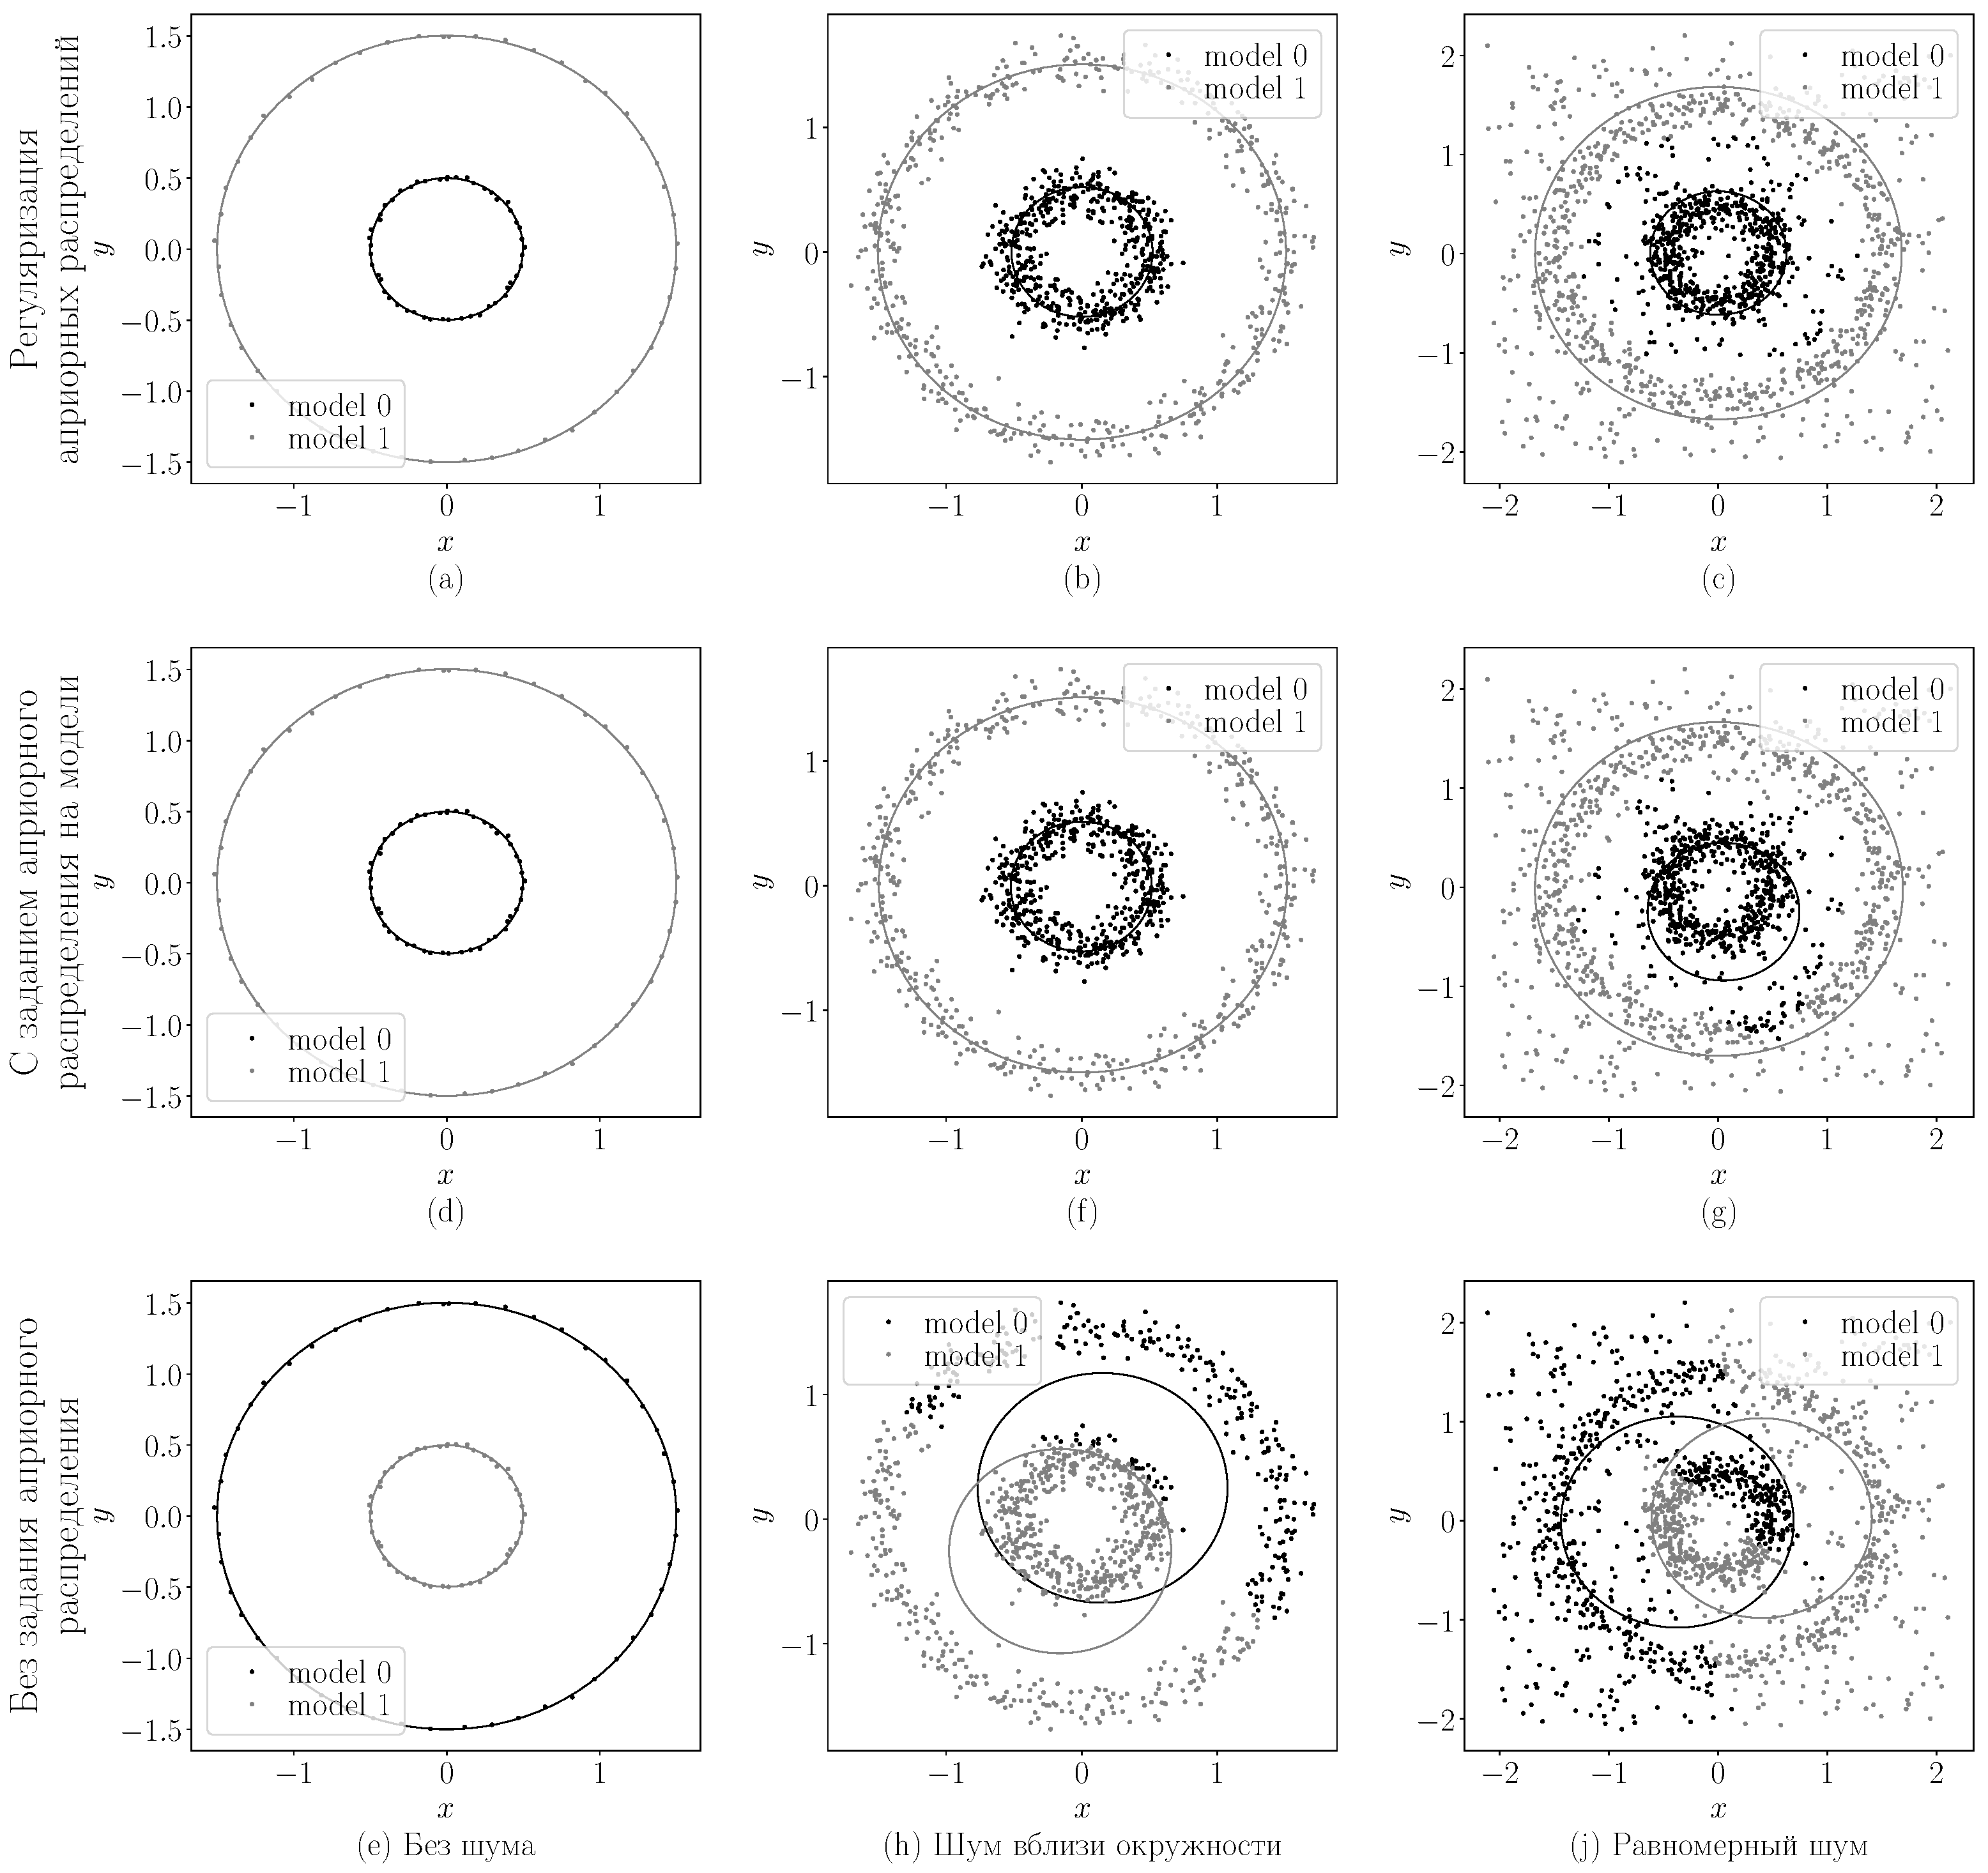
\includegraphics[width=1\textwidth]{result/experiment_synthetic}
\caption{Мультимодель в зависимости от разных априорных предположений и в зависимости от разного уровня шума: (a)--(с) модель с регуляризаций априорных распределений; (d)--(g) модель с заданными априорными распределениями на параметрах локальных моделей; (e)--(j) модель без заданных априорных предположений}
\label{experiment:1}
\end{figure}
Вычислительный эксперимент проводится на синтетической выборке, которая получена при помощи генерации двух концентрических окружностей с разным уровнем шума.

Предлагается сравнить две постановки задачи смеси экспертов: в случае когда используются априорные знания об изображении и в случае когда априорные знания отсутствуют. Причем априорные знания задаются двумя разными способами: с регуляризацией априорных распределений и без нее.

Априорные распределения на параметры локальных моделей в эксперименте было задано следующим образом:
\begin{equation}
\label{eq:ce:1}
\begin{aligned}
\mathcal{N}\left(\textbf{w}_1|\textbf{w}^{0}_{1}, \textbf{I}\right), \quad \mathcal{N}\left(\textbf{w}_2|\textbf{w}^{0}_{2}, \textbf{I}\right),
\end{aligned}
\end{equation}
где $\textbf{w}^{0}_1 = [0, 0, 0.1],\ \textbf{w}^{0}_2 = [0, 0, 2]$, что указывает на концентричность окружностей и на различность радиусов.

\begin{comment}
\begin{table}[h!t]
\begin{center}
\caption{Результаты работы мультимоделей}
\label{tb:ce:1}
\begin{tabular}{|c|c|c|c|}
\hline
	Мультимодель & Without Noise& Noise near circle& Uniform noise\\
	\hline
	\multicolumn{1}{|l|}{With prior}
	& $99/100$& $97/100$& $95/100$\\
	\hline
	\multicolumn{1}{|l|}{Without prior}
	& $68/100$& $23/100$& $7/100$\\
\hline

\end{tabular}
\end{center}
\end{table}
\end{comment}

На рис.~\ref{experiment:1} показан случайный результаты работы мультимоделей с априорными знаниями и без них. На всех картинках обе модели работала $50$ итераций. Так как сходимость мультимодели очень сильно зависит от начальной инициализации, также был проведен эксперперимент с множественным запуском мультимодели на одном и том же изображении, после чего результаты были усреднены. 

%Обе модели на каждом изображении запускались по $100$ раз. В таб.~\ref{tb:ce:1} показано сколько мультимоделей правильно отыскали обе окружности на рисунке. Как видно мультимодель с использованием априорных знаний является более стабильной, чем мультимодель, которая не использует никаких априорных знаний.

\begin{figure}[h!t]\center
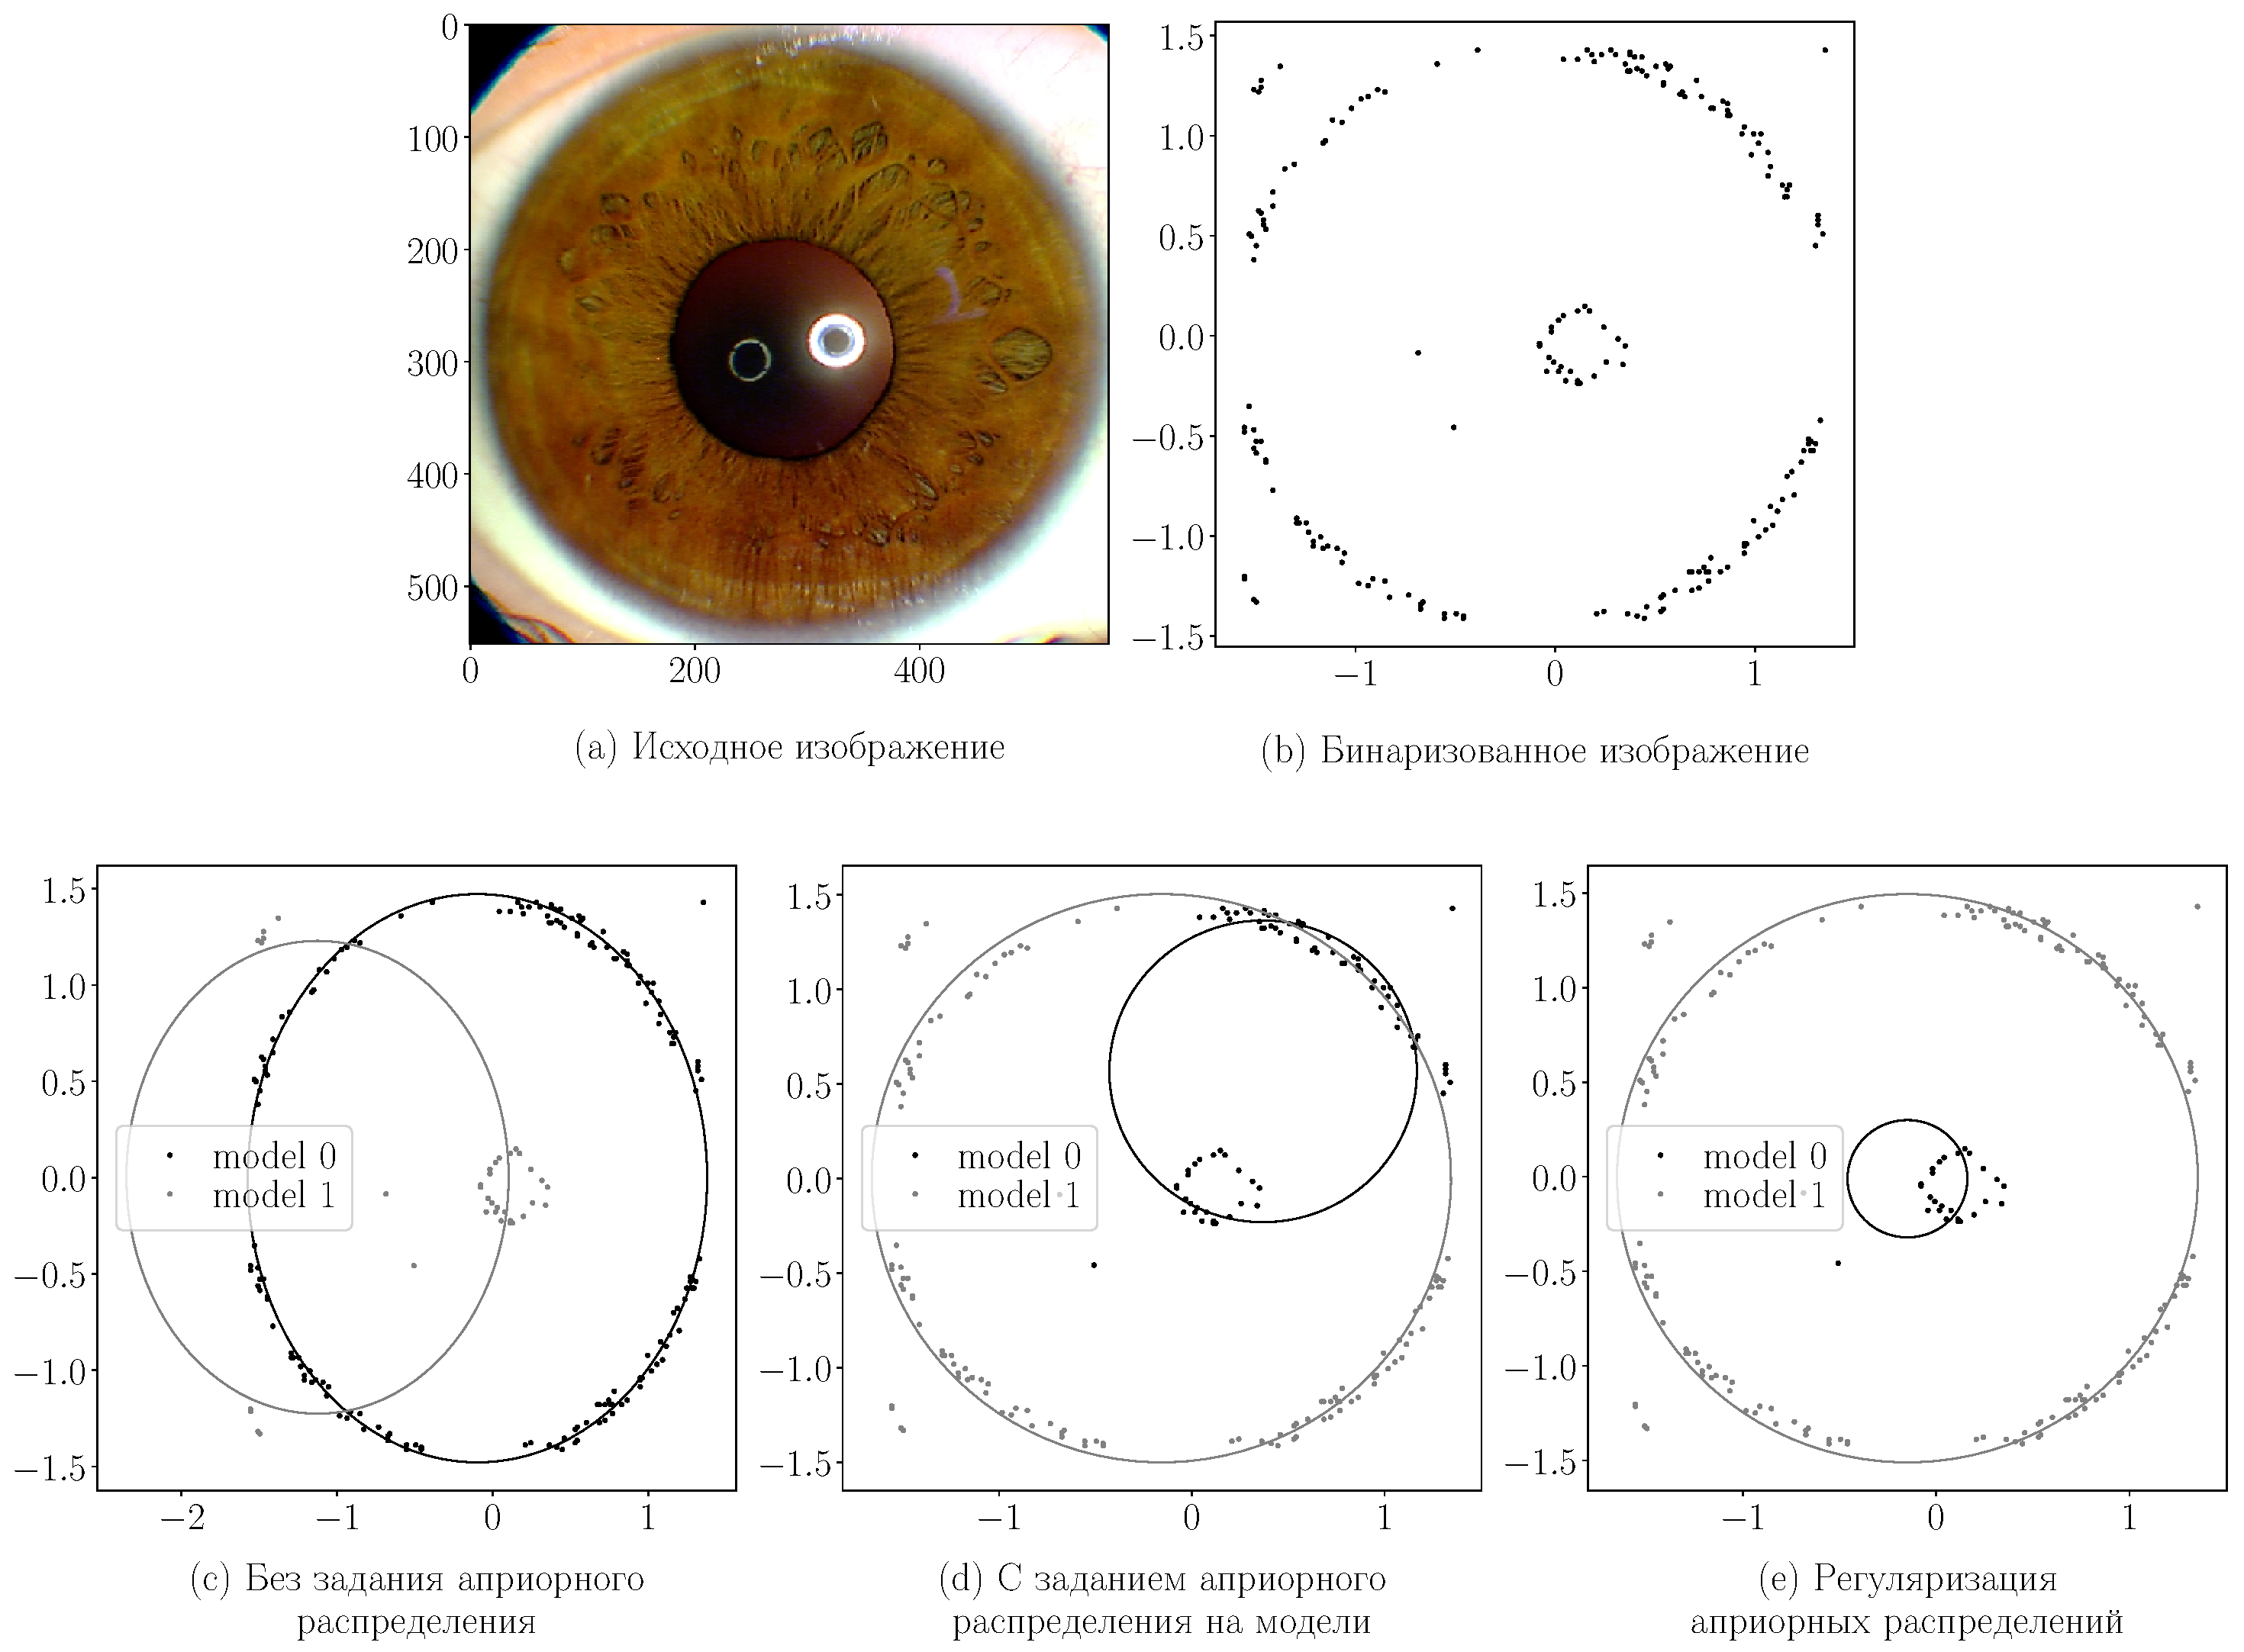
\includegraphics[width=1\textwidth]{result/experiment_real_compare}
\caption{Мультимодель в зависимости от разных априорных предположений на реальном изображении: (a) исходное изображение; (b) бинаризованое изображение; (c) мультимодель без априорных предположений; (d) мультимодель с априорными распределениями на параметрах локальных моделей; (e) мультимодель с регуляризаций на априорных распределениях параметров локальных моделей}
\label{experiment:2}
\end{figure}

\paragraph{Реальные данные.}
Проведен эксперимент на реальной выборке. В качестве данных рассматривались глаза, а точнее их предобработаное бинарное изображение с выделенным окружностями. Предлагается сравнить работу мультимоделей с разным количеством априорной информации об изображениях. Рассматривалась мультимодель в котором не было задано никаких априорных знаний. Рассматривалась мультимодель, где в качестве априорных знаний задавались априорные распределения на вектора параметров локальных моделей, также рассматривалась мультимодель, где в качестве априорных знаний дополнительно была введена регуляризация априорных распределений.


На рис.~\ref{experiment:2} показан результат работы мультимоделей с разным количеством априорной информации. В случае, когда априорные распределения не заданы мультимодель верно находит внешнюю окружность, но не находит внутреннюю окружность. В случае, когда задано априорное распределение на параметры локальных моделей качество нахождение окружностей улучшилось, но внутренняя окружность все еще найдена не верно. После добавления к заданным априорным распределениям параметров регуляризации качество мультимодели выросло, что позволило верно найти и внутреннюю окружность.

\begin{figure}[h!t]\center
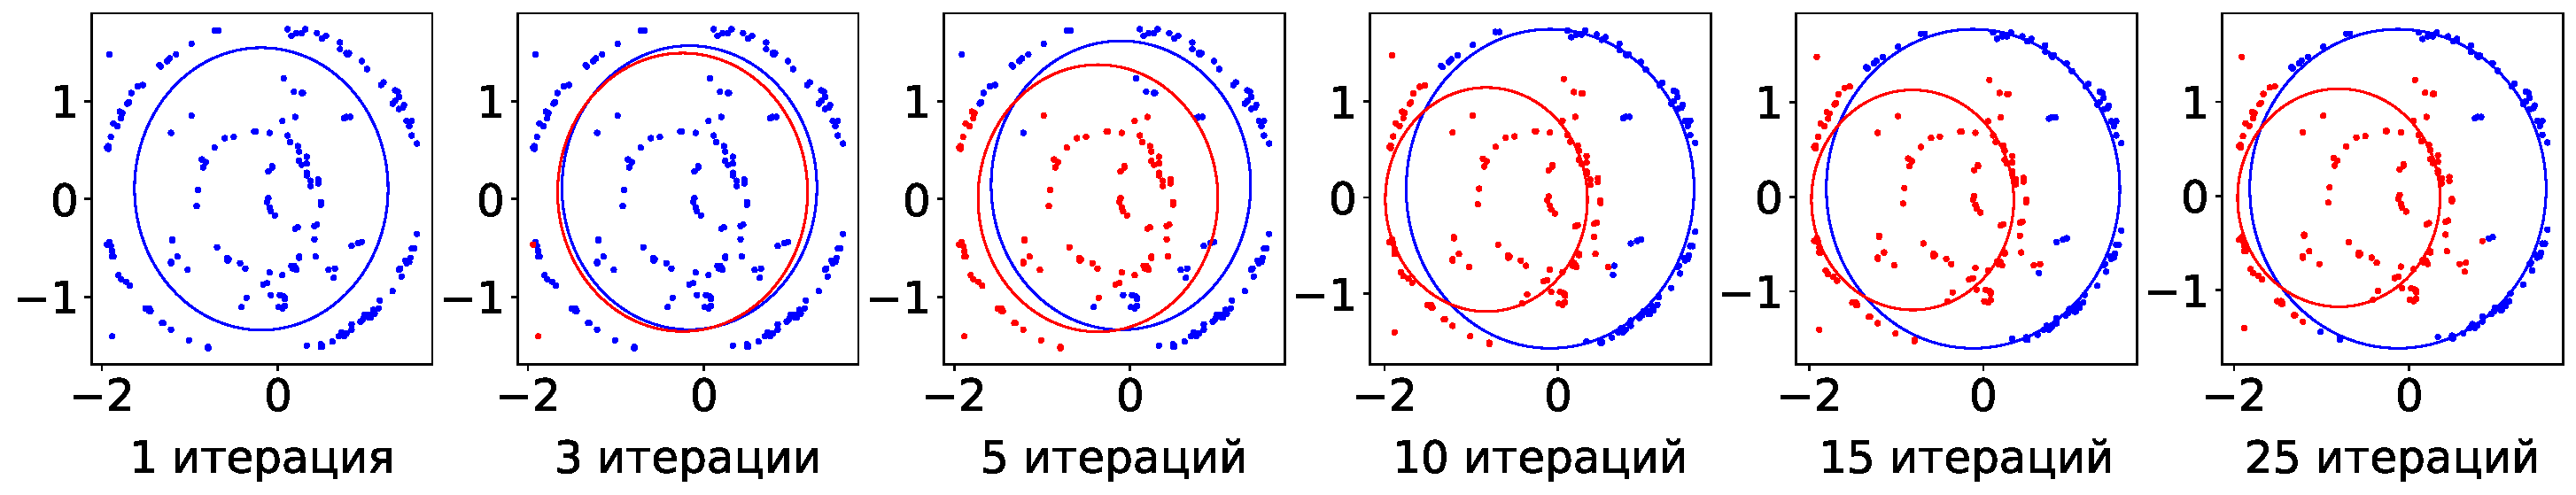
\includegraphics[width=1\textwidth]{result/experiment_real_not_prior}
\caption{Визуализация процесса обучения для мультимодели без априорных предположений: от 1й итерации до 15й итерации}
\label{experiment:3}
\end{figure}

\begin{figure}[h!t]\center
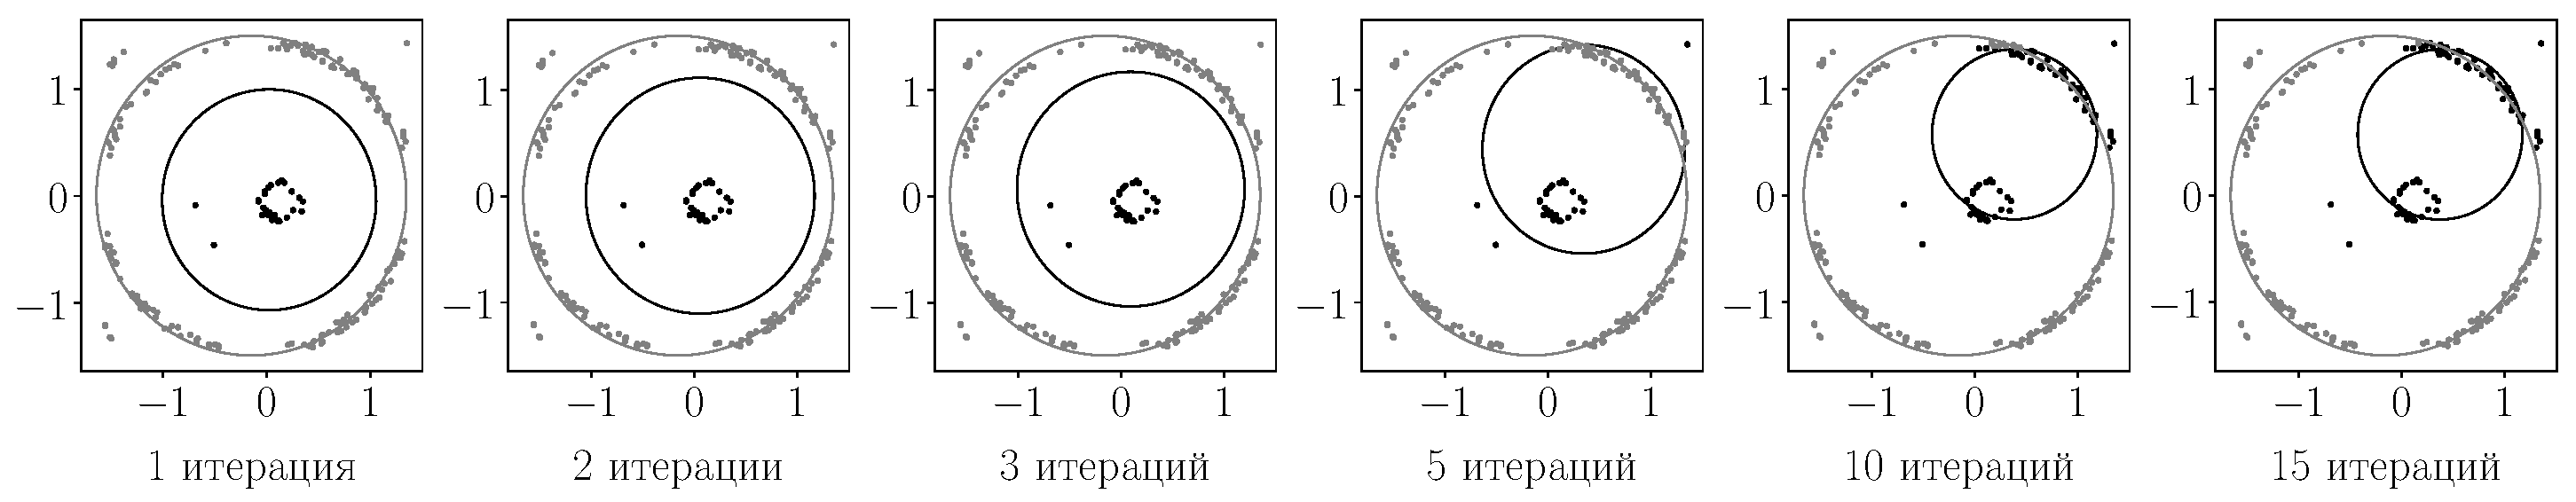
\includegraphics[width=1\textwidth]{result/experiment_real_prior}
\caption{Визуализация процесса обучения для мультимодели с априорным распределением на параметрах локальных моделей: от 1й итерации до 15й итерации}
\label{experiment:4}
\end{figure}

\begin{figure}[h!t]\center
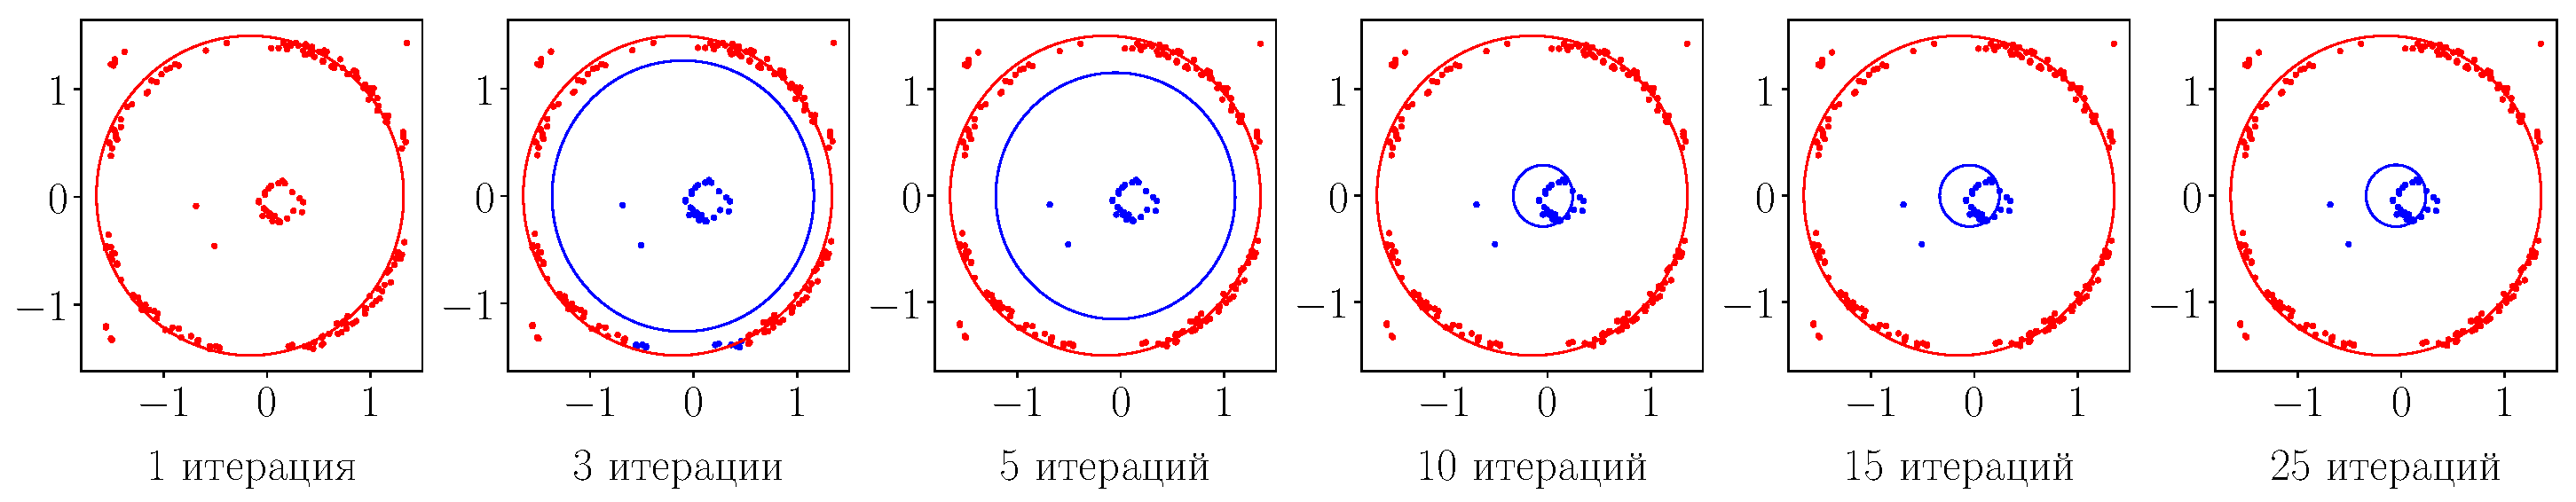
\includegraphics[width=1\textwidth]{result/experiment_real_regular}
\caption{Визуализация процесса обучения для мультимодели с заданной регуляризацией: от 1й итерации до 15й итерации}
\label{experiment:5}
\end{figure}

На рис.~\ref{experiment:3}-\ref{experiment:5} показан процесс оптимизации мультимоделей и как менялись их предсказания в процессе обучения. На рис.~\ref{experiment:3} показан процесс оптимизации для мультимодели без априорных знаний. На рис.~\ref{experiment:4} показан процесс оптимизации для мультимодели, в которой на параметры локальных моделей задано априорное распределение. На рис.~\ref{experiment:5} процесс оптимизации для мультимодели с априорным распределением на параметры локальных модели, а также регуляризация априорных распределений.

\section{Заключение}
В данной работе проведено сравнение мультимоделей в случае, когда было задано априорное распределение параметров каждой модели внутри мультимодели и в случае, когда априорного распределения не было. В качестве данных использовались изображения концентрических окружностей с разным уровнем шума. Для поиска окружностей использовались линейные модели. В качестве шлюзовой функции использовалась двухслойная нейросеть.

Как показано в эксперименте в случае, когда введены априорные знания на линейные модели, мультимодель является более точной, так как вернее находит окружности на изображениях.
%Также в случае задания априорных знаний моделей, мультимодель менее зависит от начальной инициализации, что также позволяет сказать, что модель является более устойчивой к начальной инициализации.

Также был проведен эксперимент по заданию регуляризации на априорные распределения параметров локальных моделей. В эксперименте показано, что в случае, когда регуляризация задана мультимодель находит окружности точнее.

В ходе эксперимента было показано, что модель, которая рассматривалась в работе является чувствительной к выбросам. Для решения данной проблемы предлагается рассматривать не только локальные модели, которые описывают окружности, но также и модели, которые описывают шум. 

В дальнейшем планируется улучшить мультимодель при помощи задания априорного распределения на шлюзовую функцию. Планируется рассмотреть в качестве моделей не только модели, которые описывают данные, а также модель, которая отвечает за шум в данных. Предполагается, что вероятность шума мала, поэтому важно задать априорного распределение, которое учитывало бы этот факт.

%[2, 59,12,14]

\begin{thebibliography}{99}
\bibitem{Tianqi2016}
	\textit{Chen Tianqi, Guestrin Carlos} XGBoost: A Scalable Tree Boosting System~// KDD ’16 Proceedings of the 22nd ACM SIGKDD International Conference on Knowledge Discovery and Data Mining. 2016.
	
\bibitem{Ishwaran2012}
	\textit{Chen Xi, Ishwaran Hemant} Random Forests for Genomic Data Analysis~// Genomics. 2012. Issues. 99, No 6. pp. 323--329.

\bibitem{Yuksel2012}
	\textit{Yuksel Seniha Esen, Wilson Joseph N., Gader Paul D} Twenty Years of Mixture of Experts~// IEEE Transactions on Neural Networks and Learning Systems. 2012. Issues. 23, No 8. pp. 1177–1193.

\bibitem{Shazeer2017}
	\textit{Noam Shazeer, Azalia Mirhoseini, Krzysztof Maziarz} Outrageously large neural networks: the sparsely-gated mixture-of-experts layer~// ICLR, 2017.

\bibitem{Edward2002}
	\textit{Rasmussen Carl Edward, Ghahramani Zoubin} Infinite Mixtures of Gaussian Process Experts~// Advances in Neural Information Processing Systems 14. 2002. pp. 881–888.
	
\bibitem{Jordan1994}
	\textit{M.~I.~Jordan} Hierarchical mixtures of experts and the EM algorithm~// Neural Comput., vol. 6, no. 2, pp. 181–214, 1994.
	
\bibitem{Lima2007}
	\textit{C.~A.~M.~Lima, A.~L.~V. Coelho, F.~J.~Von~Zuben} Hybridizing mixtures of experts with support vector machines: Investigation into nonlinear dynamic systems identification~// Inf. Sci., vol. 177, no. 10, pp. 2049–2074, 2007.

\bibitem{Cao2003}
	\textit{L.~Cao} Support vector machines experts for time series forecasting~// Neurocomputing, vol. 51, pp. 321–339, Apr. 2003.

\bibitem{Dempster1977}
	\textit{A. P. Dempster, N. M. Laird and D. B. Rubin} Maximum Likelihood from Incomplete Data via the EM Algorithm~// Journal of the Royal Statistical Society. Series B (Methodological), Vol. 39, No. 1 pp. 1-38, 1977.
	
\bibitem{Jordan1991}
	\textit{M.~I.~Jordan, R.~A.~Jacobs} Hierarchies of adaptive experts~// in Advances in Neural Information Processing Systems. Cambridge, MA: MIT Press, 1991, pp. 985–992.

 \end{thebibliography}

\end{document}

